\chapter{Introduction} \label{Introduction}
\todo{Enbart kommentarer, annars färdigt}

With car safety and autonomous driving being ever more prominent in our society, and ambitious visions of zero car fatalities by leading car manufacturers like Volvo, there is a growing demand for data to support these efforts. Extensive testing and research are crucial for realizing these goals. A research facility for tests like these is located just outside of Borås, owned by Research Institutes of Sweden, and opera\-ted by AstaZero. Assessments of this nature are collectively known as the New Car Assessment Programme, with the European division simply being called Euro NCAP. In addition to rating the safety performance of different vehicles, these tests also provide essential data for further development of car safety programs. To utilize the data to its maximum extent, it is essential to be able to revisit the tests, which requires accurate and reliable footage of the various test scenarios. An accurate depiction of the test and how the various vehicles compare are of essence, this is achieved when the tests are conducted in a consistent and standardized manner, implying that dynamic and autonomous footage capturing is applicable. This Bachelor thesis at Chalmers University of Technology will in joint venture with students from Penn State university develop software that enables automated video documentation of NCAP tests by the use of drones. 

\section{Background} \label{Background}
The European New Car Assessment Programme (Euro NCAP) is a comprehensive initiative that evaluates the safety of vehicles that are about to be introduced to the market. These tests are carried out globally in order to ensure accurate and unbiased assessments for the car being tested, leading to increased demand for safer cars. The vehicles are assigned a safety rating on a scale from 0-5 stars, zero stars implying that the vehicle is virtually unsafe. NCAP-tests assess the safety in several different traffic scenarios, including safety for the driver, passengers, fellow road users and pedestrians. The tests were initially conducted merely in crash scenarios, but ever since the introduction of smarter cars the tests are also performed for crash avoidance and auto-pilot assist, with plans for conducting tests for fully automated vehicles the coming decade~\cite{EuroNCAP2022EuroMobility}. 
\bigskip
\newline
To ensure the reliability and accuracy of the test results there is a need for documentation of the tests being conducted, including footage of the various scenarios. The footage of today is mostly static, either by use of stationarily situated cameras or drones following a predetermined trajectory~\cite{EuroNCAP2021EUROPEANPROTOCOL}. 
\bigskip
\newline

\section{Objective} \label{Objective}

The bachelor thesis constitutes a collaborative effort between students from Chalmers University of Technology in Gothenburg and Pennsylvania State University in State college, Pa. The joint venture aims at creating automated video documentation of a Euro NCAP test, utilizing drones. The project is conducted on behalf of AstaZero a subsidiary of Research institutes of Sweden (RISE). The final objective of the project is to deliver an application that, based on information pertaining to the moving vehicle, automatically calculates paths and proper camera angles for the drones. The position as well as the angle of the drones will be in accordance with the Euro NCAP film and photo protocol to ensure valid documentation that conforms to the already established standards~\cite{EuroNCAP2021EUROPEANPROTOCOL}.
\bigskip
\newline 

\section{Problem Statement} \label{chap:problem statement}

AstaZero is currently using a developed in-house program of their own creation called ATOS, which is an abbreviation  for Autonomous Testing Operating System \cite{AstaZero2023ATOS:Systems.}. This program allows for initiation and termination of the cars that have been assigned predetermined paths. These paths have been created manually and the cars remain in their starting positions until ATOS triggers the execution command and the cars start moving. However, this approach requires continuous manual calculation of new paths for the drones whenever a new scenario is tested, which can be tedious and time consuming. The problem at hand is therefore to develop an automated and adaptive solution for %drone path calculation,
documentation of the ongoing test,
which ultimately will enable Euro NCAP tests to be conducted at various locations with different scenarios that can be switched with ease and flexibility.
\bigskip
\newline

 Further documentation of these tests and the protocol for filming them can be found in the following papers: lane support tests~\cite{EuroNCAP2022EUROPEAN2023b}, autonomous emergency breaking in car to car tests~\cite{EuroNCAP2022EUROPEAN2023}, autonomous emergency breaking in situations where vulnerable road users are exposed ~\cite{EuroNCAP2022EUROPEANNCAPb}, and film and photo protocol~\cite{EuroNCAP2021EUROPEANPROTOCOL}. By splitting the project the following subproblems are obtained: 
\newline
%%MF \begin{itemize}
    \begin{enumerate}
        \item Research about the drones.
        \item Research about Euro NCAP tests.
        \item Create a simulation with information about the predetermined paths of the vehicles.
        \item Design the app to make it easy to use.
        \item Create the real test at AstaZero's test facility.
    \end{enumerate}

%%MF \end{itemize}
Wishes from AstaZero:
\newline
%%MF \begin{itemize}
    \begin{enumerate}
        \item Currently used drone only has 15 minutes of battery (design the solution in a way that is energy-conservative).
        \item They use many different systems, this one should be simple and easy to configure and use.
        \item Tests are not always carried out at the same position in the world, this system should support this.
    \end{enumerate}
%%MF \end{itemize}
Later during the project, AstaZero wanted to add some wishes, expanding the list. AstaZero wished to add a way to do ''dry runs'' meaning that the test ran but not the drone. This is to save battery while setting up the test and doing test runs.

\section{Demarcation} \todo{TS, Vi har j en budget att använda som vi ej gjort. Ska vi nämna det något?}\label{chap:demarcation}
Given that the framework for conducting this project is already established, the only demarcations for the project are according to the project description and software limitations as well as drone limitations. However, the project group has decided to establish some basic demarcations to further clarify the project parameters. 

\bigskip
The client, AstaZero, expressed a wish that a charging/docking station be developed by the Mechanical engineering students, as the programming part may prove to be too challenging early on in the project. However, after careful consideration, both the Chalmers and PSU groups concluded that the accumulated programming skills were sufficient. The original task therefore remained the primary focus throughout the project.
Both the groups assessed the feasibility of also constructing a charging station for the drones, but as the project continued, the time frame was not sufficient and therefore disregarded the idea. 
\bigskip
\newline
Drones of type DJI Mavic 2 Enterprise ~\cite{DJI2018MavicDJI} have been provided by the client AstaZero. Therefore the project will be conducted based on the opportunities and limitations that the hardware sets, both in terms of flying and video capturing. 
\bigskip
\newline
%Due to limited knowledge and little prior experience regarding app development, programming in Java and communication with drones presents a challenge. This implicitly means that more time has to be spent on researching, learning and troubleshooting. This will ultimately lead to less progress being made compared to working with extensive experience and knowledge.
The challenge of developing an app, programming in Java, and communicating with drones is compounded by limited knowledge and little prior experience. This means that more time will be required for research, learning, and troubleshooting. This will ultimately lead to less progress being made compared to working with extensive experience and knowledge.
\bigskip
\newline
Due to the limited experience in the subject and the restricted time frame the focus will first and foremost be to maximize efficiency and proficiency of one single assessment from the Euro NCAP tests. 
\bigskip
\newline
The drones of type DJI Mavic 2 Enterprise  have limited battery and will only be able to film for about 15 minutes before they need to recharge. This presents a challenge since a test can be longer than 15 minutes if it needs to be rerun. Instead of creating a solution for charging the drone automatically, the officials on the test track will just simply switch drones or batteries if there is not enough time to construct a charging station.
\bigskip
\newline
Further development of other tests will be implemented given that there is sufficient time. However, during the development of the first test, there will be efforts to generalize the code to make it intuitive and simple to add new tests to the program.
\bigskip
\newline
The drone in question only has one camera and uses different sensors in collaboration with built in software to avoid obstacles. For high speeds the drone might have to enable "sports mode" which deactivates some of the built in object avoidance protocols. This puts great trust in the officials performing the test to make sure that the area around the test site is clear and free of obstacles. 
\\
Furthermore, AstaZero has provided an android phone which is used for the drone controller. The application development will be limited to Android devices.
\section{Project outline}
The primary objective utilizing a DJI Mavic 2 Enterprise Zoom is to successfully capture a demonstration of the autonomous emergency braking test. To ensure that the test is conducted properly, it is essential to follow the established protocol precisely. Therefore, it is important to pay close attention to the following guidelines which according to the Euro NCAP protocol describes how the test should be captured
~\cite{EuroNCAP2021EUROPEANPROTOCOL}:
\begin{itemize}
    \item At the start of filming the car and dummy should be in view with the dummy moving towards the camera. The camera should be positioned at an angle of approximately 45 degrees to the dummy motion. When the car is about to brake, view should start to zoom in until the car has stopped.
    \item For at least half of the runs required under media films, a drone must be used in replacement of this view. Start filming following the car. When the car approaches the target, both the car and the target should be in view. The angle should be as perpendicular as possible to the car and target in order to show the action.
\end{itemize}


\begin{figure}[h!]
\centering
 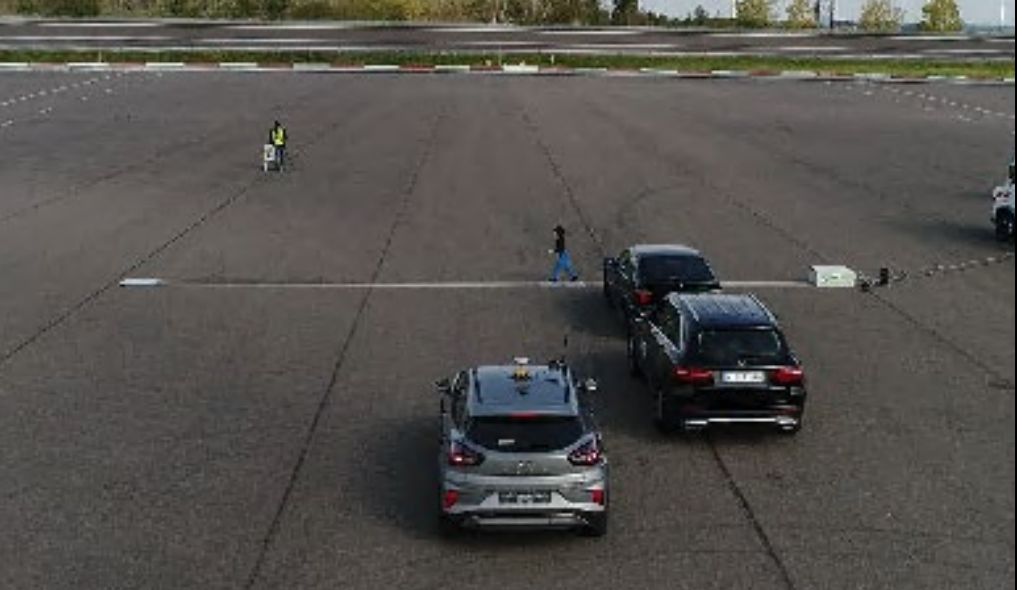
\includegraphics[width=0.65\textwidth,angle =0]{figure/45_degree_angle_of_abs_test.png}
\caption{Wide view initially.
Car and dummy in view with dummy moving towards camera. Camera angled at approximately 
45 degrees.~\cite{EuroNCAP2021EUROPEANPROTOCOL}} 
\end{figure}

%In order to attain the objective of this project, it has been divided into several subtasks. The first subtask is to ensure that the drone is capable of detecting the car with precision, enabling the gimbal to trace the car and capture it at the appropriate angle. To do this object detection is implemented. Once the car has been detected, the drone must be capable of tracking the car with use of a given path delivered from ATOS.  

To achieve the goal of this project, several subtasks have been identified. The first subtask is to implement object detection, which will allow the drone to detect the car with precision. This will enable the gimbal to trace the car and capture it at the appropriate angle.

The object detection algorithm in the app will use computer vision techniques to analyze the video feed from the drone's camera and identify the car. \todo{Här får Johan förklara mer om vilka metoder som används för att utföra detta. Vidare för det förklaras mer under ett annat kapitel}

Once the car has been detected the application will use the path provided by ATOS to guide the drone's flight path and ensure that it is following a given trajectory. This will involve calculating the drone's position relative to the car and adjusting its flight path and camera angle in real time to keep the car centered in the frame.

A simple visual representation of the objective and its operation principle is shown in figure \ref{fig:visualization} below.

\begin{figure}[H]
  \centering
  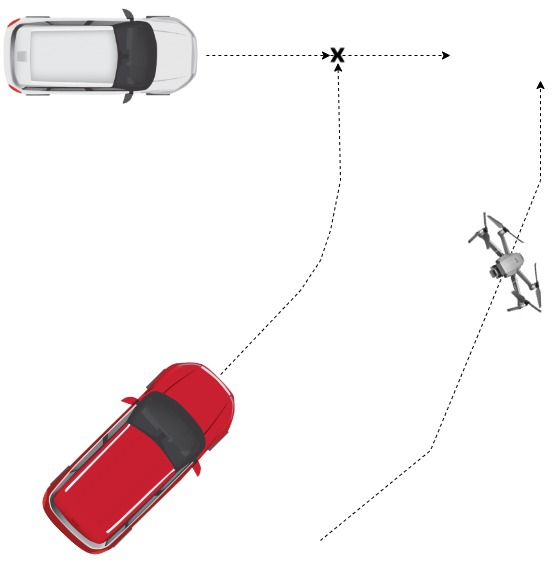
\includegraphics[width=0.75\columnwidth]{figure/traj.jpg}
  \caption{Visualization of the operation principle}
  \label{fig:visualization}
\end{figure}



